\chapter{Future Work}
\label{futureWork}

\section{Direct Improvements To Misheard Me Oronym ParseTree}
\label{section:directImprovementsToMisheardMeOronymParseTree}


Our oronyms trees display all the phonetically-matched oronyms that our users came up with. Unfortunately it also displayed a few that no human in their right mind would think of, and incorrectly weighted some others. 


\section{Places for improvement}
In some cases, our phrase-frequency metric did not accurately line up with the actual transcription frequencies from our user studies.  We believe that there are two possible reasons for this.  

\subsection{Frequency Validity}
\label{subsection: frequencyValidity}
Our frequency source data ended up being less than statisfactory. The lack of phonemic frequency data is a known defeciency in our source dictionary, UNISYN. According to the authors of the UNISYN lexicon documentation:
\begin{quote}
Unfortunately there is currently no method for distinguishing between homographs by frequency. Furthermore, it should be noted that the frequency field, as it was obtained from simple word lists, is not particularly reliable. 
\end{quote}\cite{fitt_documentation_2000} The UNISYN frequency count is based upon a large but not exhausting corpus of text.  It has some particularly glaring deficiencies in the medical arena.  We find this frustrating, because knowledge about common medical mondegreens could be used to prevent mistakes in patient's treatment plans\cite{medicalMondegreensWhenIUseAWord}. Also, it meant that the word ``colitis" wasn't in our dictionary, and we therefore couldn't use the example ``the girl with colitis goes by/the girl with kaleidescope eyes". 

Also, the fact that our program cannot distinguish between words that may be homographs (that is, words that sound different but are spelled the same) makes it improperly weight some phrases over others. For example, take the words for the animals ``bucks" and ``does".  ``Bucks" has a frequency of 1133, and ``does" has a frequency of 508386.  For reference, ``deer" has a frequency of 1896.  You can see the relative scale of these in figure ~\ref{fig:DoesBucksDeerBubbleGraph}.  It seems highly unlikely that the male and female labels for a species would be more common than the actual name of the species, given that we don't see this for sheep (sheep , 13572 , ewe , 186 , ram , 681) or horses (horse , 27559 , mare , 1055 , stallion , 644 ).  What is much more likely is that ``bucks" is getting extra hits through its meaning as a slang synonym for dollars (dollars, 8927), and ``does" is getting most of its frequency count for the 3rd person present tense of the verb ``to do".  That seems very likely, given that the frequency for the singular ``doe" is only 1077. 
\begin{figure}
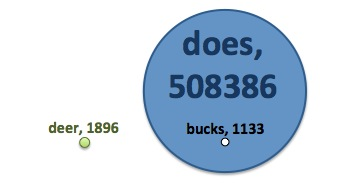
\includegraphics{DoesBucksDeerBubbleGraph.jpg}
\captionfonts
\caption[Bubble Chart comparison of Frequency for deer, does, and bucks]{Bubble Chart comparison of Frequency for deer, does, and bucks }
\label{fig:DoesBucksDeerBubbleGraph}
\end{figure}

In the future, we'd like to find a dictionary with some way of distinguishing homographs when counting frequency, and that takes a larger, more-diverse dataset into its frequency count, such as the frequency lists from the Corpus of Contemporary American English\cite{freeFreqList}.   The COCAE corpus is entirely focused on word frequency, and as such, does not contain any phonetic data.  However, it contains several different ways of determining frequency of words that overcomes some of the shortcomings we ran into trying to compare the semantically-identical words `a' and `an'.  `A' is found much for frequently than `an', but both are just as familiar.  In the UNISYN dictionary, we only have contextless frequency counts.  In the COCAE frequency dictionary, they keep two types of counts: one for how many times the word has been found, and one for how many documents is has been found in.  This way, even though `a' is found almost seven times as often than `a' overall, we know that they're equally-familiar words, because they are both found in approximately 160k corpus entries\cite{davies_word_2011}.

\subsection{Higher-order frequency data}
\label{subsection:HigherOrderFrequencyData}

Right now, our program only takes into account the frequency of standalone words, without taking their context into consideration.  In the future, we'd like to integrate n-grams into our program. N-grams are a probabilistic model of predicting the next item that will follow in a sequence, based upon frequencies of how often those N items occur in sequence in a corpus of text\cite{ngramSiteFreeLists}.  A word-level 4-gram, for example, would be a series of four words. Here are some 4-gram phrases, along with counts of how often they occur, from the Google Ngram corpus:
\begin{quote}
serve as the informational 41 \\
serve as the infrastructure 500 \\
serve as the initial 5331\\
serve as the initiating 125\\
serve as the initiation 63\\
serve as the initiator 81\\
serve as the injector 56\\
serve as the inlet 41\\
serve as the inner 87\\
serve as the input 1323\\
\end{quote} \cite{allOurNgramsAreBelongToYou}




Though we are happy with our findings, we believe that we could create even better likelihood metrics with the integration of n-grams, and would suggest this for future work. 


\section{Phoneme swapping}
\label{section:phonemeSwapping}

Often when speaking, humans substitute easier-to-say phones for more time-intensive phones.  One of the main ways that this substitution occurs is through voiced/voiceless pairs.  To “voice” a phone means to cause the vocal chords to vibrate.  “Voiced” phones are singable, whereas “voiceless” phones are not.  “Voiceless” phones are like a hiss, and simply direct streams of escaping air.  Most consonant phonemes are part of a voice/voiceless pair, such as `t' and `d'.  The word ``pretty", when spoken quickly, often uses a `d' sound instead of a `t' sound, because it's easier to say. Phones are paired when the only differences between their pronuciation is the voicing, aka, when their manner of articulation (i.e. their manner of directing air during the sound), mouth end position, and mouth start position are the same.  To view all phones in the SAMPA alphabet, along with enough information to determine whether they are pairs, see table ~\ref{sampaTable}.


\section{Melody Matcher master project}
\label{melodyMatcherMasterProject}
MisheardMe Oronym Tree is a part of the Melody Matcher suite. Melody Matcher is a semi-automated music composition support program. It analyzes English lyrics along with a melody, and alerts the composer of the locations in the song where the lyrics are not deterministically understandable. Basically, it's grammar- and spell-check for songs. This is significant, because very little research has been done specifically on the quantifiable measurement of English-language lyric intelligibility, other than our project.

\vspace{14pt}
Melody Matcher aims to replicate the human ability to identify lyrics in a song that are easily misheard. We started on this project, thinking that there would be carefully-specified research on how lyrics match melodies, mathematically. As it turned out, there was very little objective literature on the subject. Because of the lack of objective information of the subject, we had to develop our method from scratch. As we progressed through our work, we went from thinking that understandability depended only on emphasis-matching, to realizing that syllable length played a huge part as well, to realizing that there are many other musical, harmonic, and linguistic factors.
\vspace{14pt}

\subsection{Target Audience and Goals}
This program is to be used as a compositional aid by anyone who wants to write songs and make them sound good, technically. It should allow the song writer to focus on more subjective criteria of what makes a song ``good'', because it will make the structural rules of lyric composition immediately apparent.

Our hope for this project is that it will be useful to burgeoning songwriters, who have the creative spark to make wonderfully poetic lyrics, but lack the ``ear'' to match their lyrics successfully to music. It should be particularly helpful to songwriters who place a high emphasis on understandability of lyrics (such as parody song writers, or lyricists for musical theater).

Additionally, Melody Matcher will be useful for songwriters for whom English is a second language. While they may be a master lyricist in their native language, writing lyrics in English can be a particular challenge, since so much of lyric-writing is dependent upon knowing the cadence of the language you're writing lyrics in, and since English has no easily-discernible rules for emphasis placement in words.



Melody Matcher analyzes the intelligibility of song lyrics by investigating 
several root causes:


\begin{itemize} 
\item Lyric/Music emphasis mismatch, due to: 

    \begin{itemize} 
    \item Note intervals
    \item Phrase emphases
    \item Word emphases
    \end{itemize} 

\item Word ``cramming'', due to:

    \begin{itemize} 
    \item Syllable lengths that exceed that of note length
    \item Mouth movement delta time intervals
    \end{itemize} 

\item Word misidentification, due to:

    \begin{itemize} 
    \item Altered pronunciation of words
    \item Phone similarity

        \begin{itemize} 
        \item Voicing (voiced vs. voiceless)
        \item Beginning/end mouth positions
        \item Type (Plosive, Fricative, affricate, nasal, lateral, approximant, semivowel)
        \end{itemize} 
    
    \item Phone sequences with multiple syntactically-correct interpretations
    \end{itemize} 
    \end{itemize} 

The fully-implemented Melody Matcher program will eventually take into 
account all of these causes of unintelligibility. 

